\documentclass[12pt]{../notes}

% Command for Questions
%\question{}

% Command for Notes
% \note{}

% Code to create a minipage where you can type in class notes. 
%%\begin{minipage}[l][2cm][c]{\textwidth}
%\begin{comment}

%\end{comment}
%%\end{minipage}

% Begin Document
%==============================================================================
\begin{document}
% Include the Title of the Handout
\ntitle{1.4: Data Exploration}

Consider the linear model 

\[Y = \beta_0 + \beta_1X_i + \epsilon_i\]

In this example, estimates of the values of $\beta_0$ and $\beta_1$ are obtained using SAS for all four scenarios. The estimated models all have identical form, with identical measures of model goodness (which we will learn about in Handouts 2.2 and beyond). 

\[\hat{Y} = 3 + 0.5X\]


\question{Using the results of Figure \ref{fitplots}, which models are appropriate, and which are inappropriate? Why?}

\begin{figure}[H]
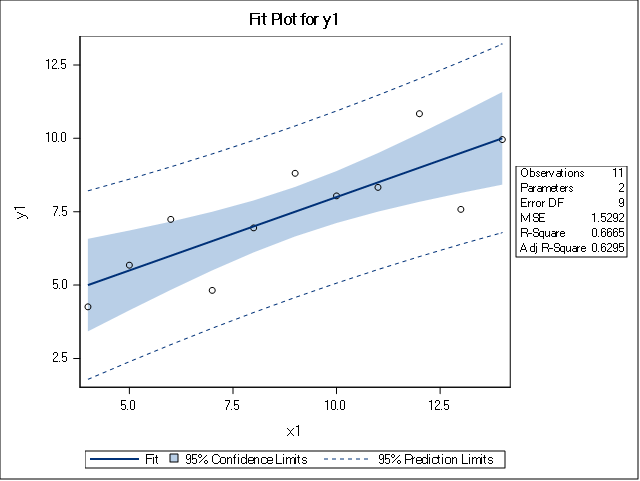
\includegraphics[width = 0.5\textwidth]{../figures/module1/fit1.png}
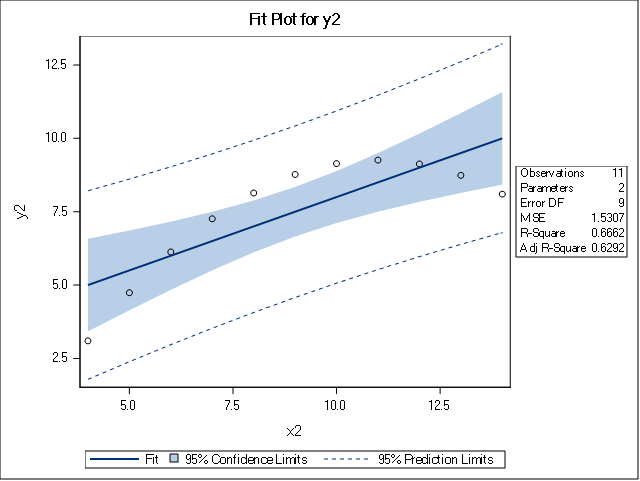
\includegraphics[width = 0.5\textwidth]{../figures/module1/fit2.png}
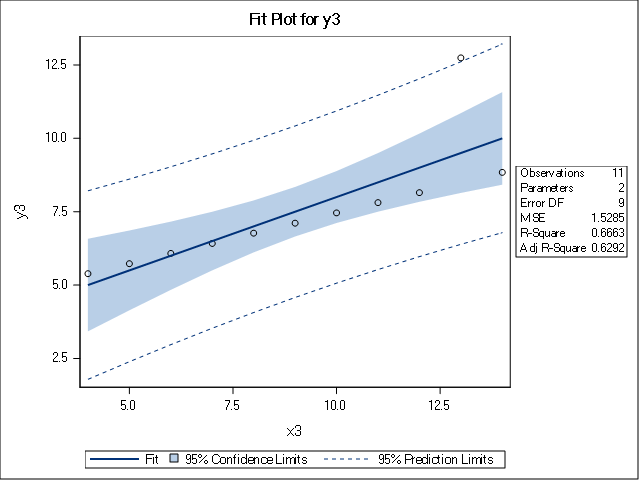
\includegraphics[width = 0.5\textwidth]{../figures/module1/fit3.png}
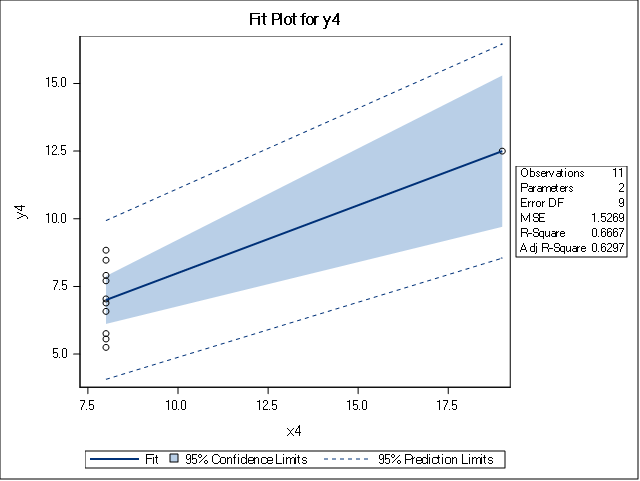
\includegraphics[width = 0.5\textwidth]{../figures/module1/fit4.png}
\caption{Plots of X vs Y, along with the estimated regression line, for Models 1-4.}
\label{fitplots}
\end{figure}

\begin{minipage}[l][6cm][c]{\textwidth}
\begin{comment}
\note{Model 1 is the only appropriate model.
\begin{itemize}
\item Model 2 (upper right) shows a non-linear relationship between X and Y. 
\item Model 3 (lower left) shows an outlier point that is making the estimated slope larger than it would otherwise be. 
\item Model 4 (lower right) shows an influential point (far right) that completely dictates the estimated slope. 
\end{itemize} }
\end{comment}
\end{minipage}

% End the Document
%==============================================================================
\end{document}